% !TEX root = knottedMain.tex
\documentclass[varwidth=\maxdimen]{standalone}

\usepackage{mathtools,amssymb,mathrsfs,dutchcal,upgreek,faktor,accents,etoolbox,multicol}
\usepackage[dvipsnames]{xcolor}
\definecolor{mygreen}{RGB}{	8,156,79 }
\usepackage{tikz,tikz-cd}
\usetikzlibrary{patterns,knots,arrows.meta,decorations.markings}
\tikzset{>={Straight Barb[scale=0.85]}}
\tikzcdset{
  cells={font=\everymath\expandafter{\the\everymath\displaystyle}},
  arrow style=tikz,
  diagrams={>={Straight Barb[scale=0.85]}},
  every label/.append style = {font = \small}
}



\begin{document}
$
\mathsf{AS}: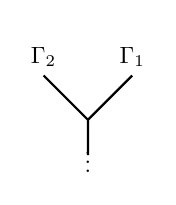
\begin{tikzpicture}[baseline=2ex,scale=0.45,every node/.style={scale=0.85}]
        \clip (-1.7,-0.6) rectangle (1.7,3.6);
        \draw
            (0,0) node[]{$\vdots$};
        \draw[thick]
            (0,0) -- (0,1) -- (-1.25,2.25) node[pos=1,above]{$\Gamma_2$}
                    (0,1) -- (1.25,2.25)  node[pos=1,above]{$\Gamma_1$};
\end{tikzpicture} 
+ 
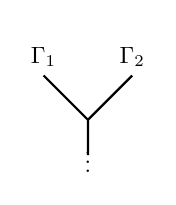
\begin{tikzpicture}[baseline=2ex,scale=0.45,every node/.style={scale=0.85}]
        \clip (-1.7,-0.6) rectangle (1.7,3.6);
        \draw (0,0) node[]{$\vdots$};
        \draw[thick]
            (0,0) -- (0,1) -- (-1.25,2.25) node[pos=1,above]{$\Gamma_1$}
                    (0,1) -- (1.25,2.25)   node[pos=1,above]{$\Gamma_2$};
\end{tikzpicture} 
=\: 0,\quad
\mathsf{IHX}: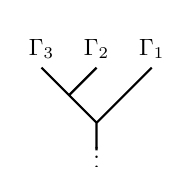
\begin{tikzpicture}[baseline=2ex,scale=0.35,every node/.style={scale=0.85}]
        \clip (-2.5,-0.6) rectangle (2.5,4.45);
        \draw (0,0) node[]{$\vdots$};
        \draw[thick]
            (0,0) -- (0,1) -- (-1,2) -- (-2,3) node[pos=1,above]{$\Gamma_3$}
                              (-1,2) -- (0,3) node[pos=1,above]{$\Gamma_2$}
                    (0,1) -- (2,3)  node[pos=1,above]{$\Gamma_1$};
\end{tikzpicture} 
-
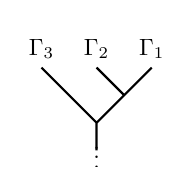
\begin{tikzpicture}[baseline=2ex,scale=0.35,every node/.style={scale=0.85}]
        \clip (-2.5,-0.6) rectangle (2.5,4.45);
        \draw (0,0) node[]{$\vdots$};
        \draw[thick]
            (0,0) -- (0,1) -- (-1,2) -- (-2,3) node[pos=1,above]{$\Gamma_3$}
                    (1,2) -- (0,3) node[pos=1,above]{$\Gamma_2$}
                    (0,1) -- (2,3)  node[pos=1,above]{$\Gamma_1$};
\end{tikzpicture} 
+ 
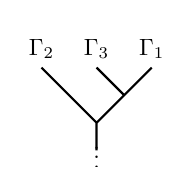
\begin{tikzpicture}[baseline=2ex,scale=0.35,every node/.style={scale=0.85}]
        \clip (-2.5,-0.6) rectangle (2.5,4.45);
        \draw (0,0) node[]{$\vdots$};
        \draw[thick]
            (0,0) -- (0,1) -- (-1,2) -- (-2,3) node[pos=1,above]{$\Gamma_2$}
                    (1,2) -- (0,3) node[pos=1,above]{$\Gamma_3$}
                    (0,1) -- (2,3)  node[pos=1,above]{$\Gamma_1$};
\end{tikzpicture} 
=\: 0.
$
\end{document}